\documentclass{ximera}

\input{../../preamble.tex}

\author{Bobby Ramsey}

\begin{document}
\begin{exercise}


\outcome{Solve inequalities.}
\tag{sign-chart}

Solve the inequality 
\[ \frac{4x+3}{3(x-5)} \leq 0 \]

by filling in the sign-chart below.

\begin{tikzpicture} 
\tkzTabInit[lgt=2,espcl=1] 
	{$x$         /1, 
	$4x+3$   /1, 
	$3$  /1,
	$x-5$       /1}% 
	{  , $-\dfrac{3}{4}$ , $5$ ,  }% 
\tkzTabLine{ ,   , t ,   , t ,   ,}
\tkzTabLine{ ,   , t ,   , t ,   ,}
\tkzTabLine{ ,   , t ,   , t ,   ,  }
\end{tikzpicture} 

The solution is: \[ \left[  \answer{-\frac{3}{4}} \, , \, \answer{5} \right)  \] 
\end{exercise}
\end{document}